\documentclass{report}

\usepackage[a4paper, total={6in, 8in}, margin=1in,footskip=0.25in]{geometry} \usepackage{amsmath, amsthm, amssymb, booktabs, chemfig, graphicx, gensymb, float, pgfplots, setspace, siunitx, tabularray}
\usepackage{tabularray}
\usepackage[hidelinks]{hyperref}

\renewcommand{\familydefault}{\sfdefault}
\newcommand{\asin}{\sin^{-1}}
\newcommand{\acos}{\cos^{-1}}
\newcommand{\atan}{\tan^{-1}}
\newcommand{\ta}{\theta}

\setlength{\parindent}{0pt}
\setlength{\parskip}{0.8em}

\pgfplotsset{compat=1.18}

\graphicspath{ {.././Images/} }

\title{\Huge Year 12 Physics - Module 7}
\author{L. Cheung}

\tolerance=1
\emergencystretch=\maxdimen
\hyphenpenalty=10000
\hbadness=10000

\begin{document}
	\maketitle
	\tableofcontents
\newpage

\chapter{Investigations}

	\section{Investigation 1: Speed of Light Investigations}
	
		\textbf{Summarise the historical and contemporary methods used to determine the speed of light and explain its current relationship to the measurement of time and distance.}

			\subitem Galileo attempted to measure the speed of light by using lantern signals across a large distance and calculating the delay over the gap. However, varying human reflexes and the primitive time measuring equipment available inhibited any recordings taken.

			\subitem Later, Romer used the eclipses of Jupiter's moon Io to estimate the speed of light. Romer observed that the time between the eclipses was not constant. Using the assumption that the orbital period of Io was not changing, he deduced that the variation was due to changes in the difference in distance between Jupiter and Earth. From his observations, Romer found the speed of light to be 226,663 km/s, 24.4\% lower than its actual value.

			\subitem Fizeau used an experiment where a toothed wheel interfered with a light source that reflected off a mirror a great distance away. By adjusting the rotational velocity of the wheel, the reflected light may or may not have been reflected.

			\subitem Foucault's experiment used a similar setup, however used a rotating mirror instead of a toothed wheel. By analysing the angle between the light source and the light received, Foucault could determine the speed of light.

			\begin{align*}
				c &= \frac{d}{t} = \frac{d}{\frac{\Delta \theta}{\omega}} = \frac{d \omega}{\Delta \theta}
			\end{align*}

			\subitem Using Maxwell's discovery on electromagnetism in the 1860s, Rosa and Dorsey derived a formula using the electric permittivity and magnetic permeability constants to calculate the speed of light.

			\begin{align*}
				c = \frac{1}{\sqrt{\epsilon \mu}}
			\end{align*}

		
\newpage

	\section{Investigation 2: Spectral Analysis}
	
		\textbf{Aim}: To determine the emission spectra of various elements

		\subsubsection{Materials}
		
			\begin{itemize}
				\item Spectroscope
				\item Spectral lamps with:
					\begin{itemize}
						\item Hydrogen
						\item Helium
						\item Neon
						\item Oxygen
						\item Mercury
					\end{itemize}
				\item Spectral lamp support
				\item Spectral lamp power supply
			\end{itemize}

		\subsubsection{Risk Assessment}

			\begin{table}[H]
				\setstretch{1.25}
				\centering
				\begin{tabular}{p{7cm}|p{7cm}}
					\textbf{Hazard} & \textbf{Precaution} \\ \hline
					High voltage power pack & Turn off when not in use, do not touch contact points \\
					Cuts from glass & Check spectral lamp before use, keep away from edge of table to prevent dropping \\
					Burns from UV light & Don't observe directly, only view via spectrometer
					
				\end{tabular}
			\end{table}

		\subsubsection{Method}
			\begin{enumerate}
				\item Prepare spectral support and power supply at 400V
				\item Insert hydrogen spectral
				\item Use spectrometer to observe emission spectrum and record wavelengths using chart on spectrometer
				\item Repeat steps 2-3 with helium, neon, sulfur, and mercury
				\item Record results
			\end{enumerate}

		\subsubsection{Results}
			\begin{table}[H]
				\centering
				\setstretch{1.25}
				\begin{tabular}{p{3cm}|p{10cm}}
					\textbf{Element}	& \textbf{Result}			\\ \hline
					Hydrogen		& Bright pink				\\
					Helium			& Red, orange, yellow			\\
					Neon			& Red, orange				\\
					Oxygen			& Pale blue white			\\
					Mercury			& Blue-green				\\
				\end{tabular}
			\end{table}

\newpage

	\section{Investigation 3: Diffraction of Light}
	
		\textbf{Summarise your qualitative analysis of light diffraction, including the experimental setup, observations, and what these phenomena demonstrate about the wave properties of light.}

			Light diffraction is the spreading out of a wave when passing around an obstacle. The scattering process changes the direction of propagation and causes the diffracting object to act as a secondary source of propagation. The degree of this direction change depends on the obstacle's size relative to that of the wavelength.

			Waves passing through a slit a relative size to its wavelength experience diffraction that creates a repeating pattern with alternating bright and dark points. Huygen's wave model of light proposed that when a wave reaches an opening, its wavefront becomes many individual points each emitting their own wavelets. As a result, waves passing through a slit will propagate outwards from the slit.

			Diffraction through two slits creates two secondary wave sources that interact constructively or destructively to produce alternating minima and maxima of diffraction. The intensity of light decreases away from the centre line.

			Young's double slit experiment involved passing a monochromatic light source through two narrow slits separated by a given distance. The results supported the wave model of light, where a particle based model could not account for the pattern produced.
				
			\begin{figure}[H]
				\centering
				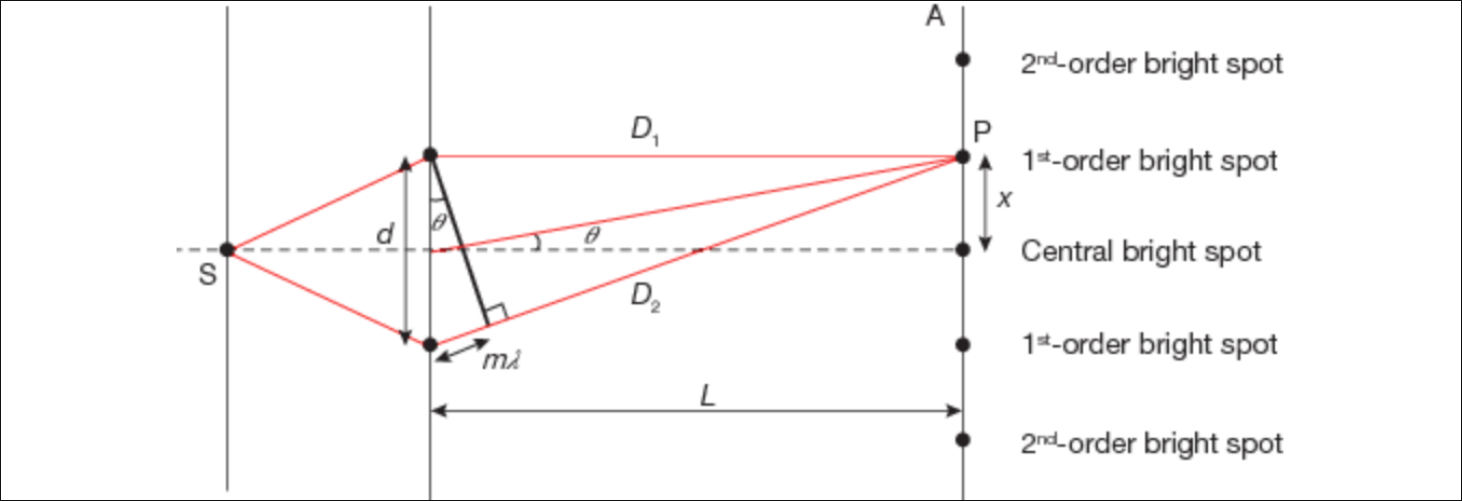
\includegraphics[width=15cm]{young_double_slit.png}
			\end{figure}


\newpage

	\section{Investigation 4: Interference and Diffraction}

		\textbf{Aim}: To observe the diffraction and interference of light using diffraction gratings
		\subsubsection{Materials}

			\begin{itemize}
				\item Laser pointer
				\item A diffraction grating set
				\item Meter ruler or tape measure
			\end{itemize}

		\subsubsection{Risk Assessment}
		
			\begin{table}[H]
				\setstretch{1.25}
				\centering
				\begin{tabular}{p{7cm}|p{7cm}}
					\textbf{Hazard} & \textbf{Precaution} \\ \hline
					Retina burns & Do not directly look at laser light \\
					Dropping equipment & Handle with caution, keep secure on table

				\end{tabular}
			\end{table}
		
		\subsubsection{Method}

			\begin{enumerate}
				\item Use supports such as retort stands to set up the laser pointer so that it shines perpendicularly onto a screen, wall, or board at least one meter away.
				\item Mount the diffraction grating directly in front of the laser pointer so that a regular row of dots appears on the screen.
				\item Measure the values of $x$ and $L$, and record these in your results table, along with the $N$ value for your grating.
				\item Repeat this procedure for each grating of different $N$ value.
				\item Analyse the data to determine the wavelength of the laser pointer.
			\end{enumerate}

		\subsubsection{Results}

			\begin{table}[H]
				\centering
				\setstretch{1.25}
				\begin{tabular}{p{4cm}|p{2cm}|p{2cm}|p{2cm}|p{2cm}}
					Slit separation $d$ (m)		& $x$ (m)	& L (m)		& $\lambda$ (m) 		& $\lambda$ (nm)	\\ \hline
					$100 \times 10^{-6}$		& 0.034		& 5.44		& $6.25 \times 10^{-7}$		& 625			\\
					$200 \times 10^{-6}$		& 0.016		& 5.44		& $5.88 \times 10^{-7}$		& 588			\\
					$300 \times 10^{-6}$		& 0.011		& 5.44		& $6.07 \times 10^{-7}$		& 607			\\
				\end{tabular}
			\end{table}
			
			Slit separation 1
			\begin{align*}
				\text{At very small angles, } \sin{\theta} = \tan{\theta} \\
				d \sin{\theta} &= m \lambda \\
				\sin{\theta} = \frac{m \lambda}{d} &= \frac{x}{L} \\
				\lambda &= \frac{dx}{L} \\
					&= \frac{100 \times 10^{-6} \times 0.034}{5.44} \\
					&= 6.25 \times 10^{-7} \\
			\text{Actual $\lambda$ of Ne-He laser} &= 6.328 \times 10^{-7}
			\end{align*}

			Slit separation 2
			\begin{align*}
				d \sin{\theta} &= m \lambda \\
				\sin{\theta} = \frac{m \lambda}{d} &= \frac{x}{L} \\
				\lambda &= \frac{dx}{L} \\
					&= \frac{200 \times 10^{-6} \times 0.016}{5.44} \\
					&= 5.88 \times 10^{-7} \\
			\text{Actual $\lambda$ of Ne-He laser} &= 6.328 \times 10^{-7}
			\end{align*}

			Slit separation 3
			\begin{align*}
				d \sin{\theta} &= m \lambda \\
				\sin{\theta} = \frac{m \lambda}{d} &= \frac{x}{L} \\
				\lambda &= \frac{dx}{L} \\
					&= \frac{300 \times 10^{-6} \times 0.011}{5.44} \\
					&= 6.07 \times 10^{-7} \\
				\text{Actual $\lambda$ of Ne-He laser} &= 6.328 \times 10^{-7}
			\end{align*}

\newpage

	\section{Investigation 5: Polarisation and Malus's Law}
	
		\textbf{Aim}: To observe plane polarisation of light using polarising filters, and to verify Malus' Law

		\subsubsection{Materials}
		
			\begin{itemize}
				\item Torch
				\item Lux meter
				\item 2 polarising filters
				\item A protractor
				\item Retort stand
				\item Bosshead
				\item Clamp
			\end{itemize}

		\subsubsection{Risk Assessment}
		
			\begin{table}[H]
				\centering
				\setstretch{1.25}
				\begin{tabular}{p{7cm}|p{7cm}}
					\textbf{Hazard}			& \textbf{Precaution}		\\ \hline
					Eye damage from torch		& Do not look directly at light source \\
					Burning				& Do not touch torch when in use. Allow cooling time when necessary
				\end{tabular}
			\end{table}

		\subsubsection{Method}
			
			\begin{enumerate}
				\item Attach polarising filters to retort stand using bosshead
				\item Attach torch above the polarising filters using bosshead and clamp facing down
				\item Place lux meter below the polarising filter, lining up with the torch
				\item Remove external light sources
				\item Record the lux where the polarising filters have angles of 0, 30, 45, 60, 90 degrees.
			\end{enumerate}

		\subsubsection{Results}
		
			\begin{table}[H]
				\centering
				\setstretch{1.25}
				\begin{tabular}{p{6cm}|p{5cm}|p{5cm}}
					\textbf{Angle between filters (degrees)}& \textbf{Measured intensity (lux)}	& \textbf{Calculated Intensity (lux)}		\\ \hline
					0					& 175					& 175					\\
					30					& 132					& 131					\\
					45					& 91					& 87.5					\\
					60					& 57					& 43.8					\\
					90					& 20					& 0					\\
				\end{tabular}
			\end{table}

			\begin{figure}[H]
				\centering
				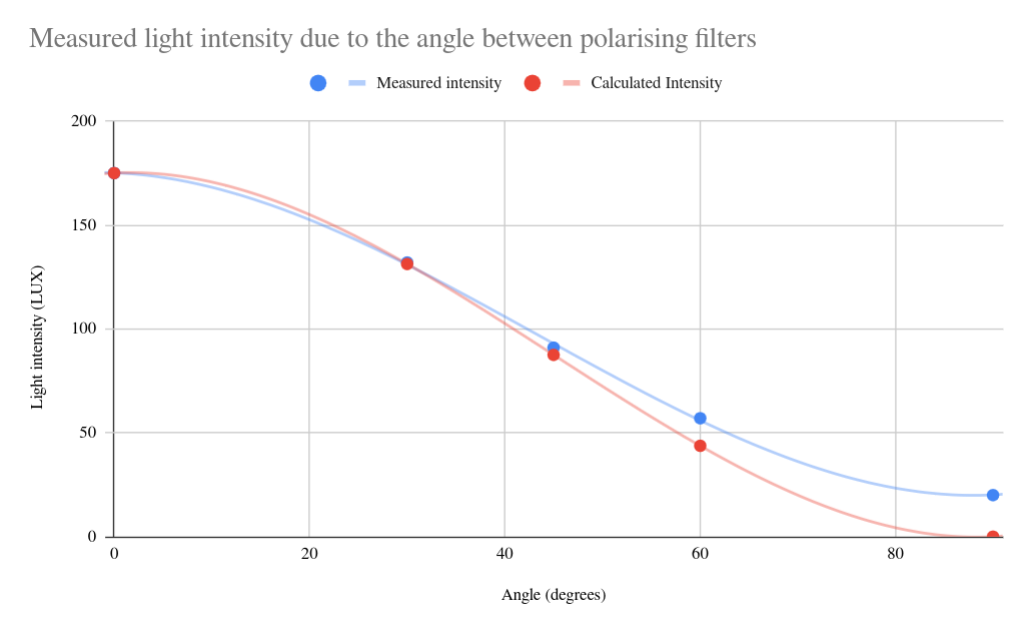
\includegraphics[width=15cm]{prac_5_graph.png}
			\end{figure}

\newpage

\chapter{Review Questions}

	\section{Set 1}
		\begin{enumerate}
			\item B
			\item D
			\item B
			\item C
			\item A
			\item \textbf{Figure 8.11 shows the emission spectrum of sodium}
				\begin{enumerate}
					\item \textbf{Describe an experiment that could be used to examine the emission spectrum of an element.}
						\subitem The spectral lamp experiment can be used to observe the emission spectrum of an element. Running high voltage current through a spectral lamp containing a specific element will emit a bright spectrum that can be split into wavelengths by a prism or a spectrocope.

					\item \textbf{Explain how emission spectra can be used to identify the elements in a sample?}
						\subitem A complete emission spectra can be analysed to find the lines in the black body spectrum and comparing that with the spectra of known elements.

					\item \textbf{If sodium was present in the atmosphere of the Sun, how would it affect the emission spectra of the Sun?}
						\subitem If sodium is present, the Sun's emission spectrum will have lines at 589 nm to 590 nm.
				\end{enumerate}

			\item \textbf{Outline one method that has been used to measure the speed of light}
				\subitem The speed of light light has been measured by Hertz who used an induction coil to produce a spark of a particular frequency. A spark gap was placed such that it would interact with the produced electromagnetic waves. By adjusting the position of the spark gap to maximise its intensity, the wavelength can be measured. Then, the formula $v=f \lambda$ can be used to determine the velocity of light.

			\item \textbf{About half of the visible stars in the sky are binary star systems, which consist of two stars orbiting each other. Consider two stars of similar mass in a binary system that has its orbital plane almost parallel to the line of sight from the Earth. Each of the hydrogen atomic absorption lines in the stellar spectrum of the binary star system are observed to split into two lines of slightly different frequency and recombine to a single line every four days.}

				\begin{enumerate}
					\item \textbf{Explain why the motion of the stars would cause the atomic absorption lines in the stellar spectra to change in this way.}
						\subitem The light from the stars will become red or blue shifted depending on each star's velocity relative to the viewer. As the hydrogen atomic absorption lines split, the stars rotate out of alignment with the Earth. One star moves away from the Earth, becoming redshifted and resulting in a longer wavelength, whereas the other star moves towards the Earth and its emitted light becomes blueshifted. When the stars are travelling perpendicularly to the Earth, ie. they are in alignment with the Earth, there is no relative motion and hence no red or blue shifting effect, creating a single line on the spectrum.

					\item \textbf{Determine the orbital period of this binary star system.}
						\subitem 8 days.

					\item \textbf{Explain why some non-hydrogen absorption lines from the binary system move back and forth around a specific frequency periodically but do not split and recombine like the hydrogen lines.}
						\subitem In order for the absorption line to split, the element blocking the wavelength must be present in both stars. If it only present in one star, then a single line will be observed, shifting as it is red or blue shifted.
				\end{enumerate}

			\item \textbf{Maxwell used his equations of electromagnetism to predict the existence of electromagnetic waves.}

				\begin{enumerate}
					\item \textbf{Explain how an electromagnetic wave can be produced.}
						\subitem An electromagnetic wave can be produced by oscillating charged particles. This creates a change in electric field that produces a change in magnetic field that is perpendicular to the charge movement.

					\item \textbf{Describe the structure of electromagnetic waves in terms of electric and magnetic fields.}
						\subitem Electromagnetic waves consist of electric and magnetic fields travelling perpendicular to each other.

					\item \textbf{If the source of an electromagnetic wave was removed, would the existing waves produced by the source continue to propagate? Justify your answer.}
						\subitem If the source is removed, the electromagnetic wave will continue to move. This is due to electromagnetic waves being self-propagating as the change in magnetic and electric fields cause each other.
				\end{enumerate}

			\item \textbf{Explain how an examination of the light from a star can be used to provide information on three physical properties of the star.}

				\subitem The gaps in the absorption spectrum of a star can show what elements are present in the star. A star's nucleus produces all wavelengths of light, however some are absorbed by the elements in the star and become gaps in the spectrum that can be analysed to determine the chemical composition of the star.

				The translational velocity of a star can also be determined by observing red and blue shifting patterns in the spectrum. The line will appear to move left and right, and this change in wavelength can be used to calculated velocity relative to the Earth and hence translational velocity.

				If the star has high density, more collisions occur between atoms and furthermore between electrons. This produces variations in energy of the electrons that blurs the lines on the absorption spectrum.
		\end{enumerate}

	\section{Set 2}
	
		\begin{enumerate}
			\item B
			\item C
			\item D
			\item A
			\item C
			\item \textbf{Explain why light is refracted, using:}
				\begin{enumerate}
					\item \textit{Huygens' wave model}
						\subitem Huygens' wave model stated that every point on the wavefront would act as source for  secondary wavelets. As the wavefront enters another medium, one part of the wavefront is affected first. This part of the wavefront is therefore sped up or slowed down depending on the medium the wave enters.

					\item \textit{Newton's particle model}
						\subitem Newton proposed that a force acted on each particle of light as they entered a new medium. When approaching the new medium, the particles would experience a force that would cause the beam to be refracted towards the normal.
				\end{enumerate}
			
			\item \textbf{In an experiment shown in Figure 9.16, unpolarised light is incident upon a pair of polaroid filters which have their polarisation axes at an angle with respect to each other. The transmitted light was found to have an intensity of 10\% of the incident light intensity.}
				\begin{enumerate}
					\item \textit{Explain the difference between unpolarised and plane-polarised electromagnetic waves.}
						\subitem Unpolarised electromagnetic waves have electric fields that oscillate in all directions perpendicular to wave velocity, whereas plane-polarised electromagnetic waves have electric fields that oscillate in one plane only.

					\item \textit{Find the angle ($\theta$) between the axes of polarisation of the two polaroid filters}

						\begin{align*}
							I_1 &= \frac{1}{2} I_0 \\
							I &= I_1 \cos^2{\theta}  = \frac{1}{2} I_0 \cos^2{\theta} \\
							I &= 0.1 \times I_0 \\
							\cos^2{\theta} &= 0.2 \\
							\cos{\theta} &= \sqrt{0.2} \\
							\theta &= \acos{\sqrt{0.2}} \\
							&\approx 63.3 \degree
						\end{align*}

				\end{enumerate}

			\item \textbf{When laser light of wavelength 630 nm is passed through a pair of slits, the first maxima on each side of the central maxima are found to be 12 cm apart from each other on a screen 4 m form the slits}
				\begin{enumerate}
					\item \textit{Why is laser light rather than light from an incandescent lamp used for interference experiments like this?}
						\subitem Laser light is used because interference patterns are most obvious when monochromatic (one coloured) light is used. Therefore, lasers producing one wavelength of light are most appropriate for interference experiments.

					\item \textit{What is the separation between the slits?}

						\begin{align*}
							d \sin{\theta} &= m \lambda	\\
							d &= \frac{m \lambda}{\sin{\ta}} 	\\
							  &= m \times 630 \times 10^{-9} \times \sin{\ta} \\
							  &= m \times 630 \times 10^{-9} \times  \frac{4}{0.06} \\
							  &= 42 \; \mu m
						\end{align*}

					\item \textit{If the double slits were replaced with a diffraction grating with a slit separation one-quarter of the double-slit separation, how would the interference pattern change?}
						\subitem The diffraction grating would be sharper and the light would have a higher intensity. As well as this, the separation between maxima would be four times further.
				\end{enumerate}

			\item \textbf{Evaluate the importance of polarisation of light to the development of the wave model of light}
				\subitem The polarisation of light created inaccuracies with the assumption of light as a particle. The process allowed some light to pass through and if light were a particle either all or none of it would pass. Furthermore, the development evolved the understanding of light as a wave, demonstrating that the compression wave theory proposed by Huygens was incorrect.

			\item \textbf{A diffraction grating is used to investigate an atomic spectrum which is is known to contain of wavelength of 430 nm and one other longer wavelength. In the interference pattern produced by the grating, the fourth-order maxima of the 430 nm line is observed to fall at the same place as the third maxima of the longer wavelength line.}

				\begin{enumerate}
					\item \textit{Sketch a qualitative diagram to show the intensity of the interference pattern that would be produced by the grating. Include the first three maxima of the longer wavelength and the first four maxima of the shorter wavelength. Label the short wavelength maxima and long wavelength maxima}

					\item \textit{Find the wavelength of the second line emitted from the atomic spectrum}
						\begin{align*}
							\lambda_\text{long} = \frac{4 \times 430 \times 10^{-9}}{3} \approx 573.3 \; nm
						\end{align*}
				\end{enumerate}

		\end{enumerate}

	\section{Set 3}

		\begin{enumerate}
			\item D
			\item C
			\item C
			\item A
			\item A
			\item \textbf{The Sun has a surface temperature of 5778 K, yet to a good approximation it can be treated as a perfect black body.}
				\begin{enumerate}
					\item \textit{What do physicists mean when they talk about a "perfect black body"?}
						\subitem A perfect black body absorbs and re-emits all electromagnetic waves no matter the wavelength.

					\item \textit{Determine the wavelength and frequency at which the Sun emits the greatest intensity electromagnetic radiation}
						\begin{align*}
							\lambda_\text{max} &= \frac{b}{T} \\
									   &= \frac{2.898 \times 10^{-3}}{5778} \\
									   &\approx 5.02 \times 10^{-7} \; m
						\end{align*}
						\begin{align*}
							f &= \frac{c}{\lambda} \\
							  &= \frac{3.00 \times 10^8}{5.02 \times 10^{-7}} \\
							  &\approx 5.98 \times 10^{14}
						\end{align*}
				\end{enumerate}

			\item \textbf{This question refers to Figure 10.10}

				\begin{enumerate}
					\item \textit{Explain why the data shown in Figure 10.10 caused concern to physicists in the late 19th century}
						\subitem When the classical electromagnetic wave model of light was applied to the black body radiation curve, it predicted that black bodies should emit an infinite amount of energy at high frequencies.

					\item \textit{Plank solved the black-body problem by making assumptions that Einstein built upon to produce a new model of light. Compare Einstein's model of light with the classical electromagnetic wave model.}
						\subitem In the wave model, energy of a wave is distributed evenly throughout the wave and is related to the wave's amplitude. Einstein redefined light as a stream of particles with an energy $E=hf$. Here, energy was quantised rather than distributed and light intensity according to Einstein was related to the number of photons and the energy of each photon.
				\end{enumerate}

			\item \textbf{Experiments with the photoelectric effect show that electrons are only emitted from a metal surface when the incident light has a frequency greater than a specific threshold frequency.}
				
				\begin{enumerate}
					\item \textit{Outline why this observation could not be explained by the classical wave model of light.}
						\subitem The classical wave model of light stated that the power of a wave is spread throughout the entire wave, and it carried energy that would liberate the electrons. However, this assumed that electrons could be liberated at all wave frequencies provided there was enough energy, which was not the case.
					
					\item \textit{Outline how the photon model can be used to explain this observation.}
						\subitem The photon model assumes that light consists of a flow of photons that each contain an amount of energy at a specific wavelength. The photon energy is determined by the frequency of light ($E = hf$), therefore only frequencies above the threshold value will be able to liberate electrons from the surface

					\item \textit{If a metal had a work function of 4 eV, what would be its threshold frequency?}

						\begin{align*}
							E &= 4 \times 1.602 \times 10^{-19} \\
							  &= 6.408 \times 10^{-19} \; J
						\end{align*}
						\begin{align*}
							E &= hf \\
							f &= \frac{E}{h} \\
							  &= \frac{6.408 \times 10^{-19}}{6.626 \times 10^{-34}} \\
							  &= 9.67 \times 10^{14} \; Hz
						\end{align*}

				\end{enumerate}

			\item \textbf{This question refers to the apparatus illustrated in Figure 10.11}

				\begin{enumerate}
					\item \textit{Explain how the apparatus in Figure 10.11 can be used to determine the total photocurrent for a specific light intensity and wavelength.}
						\subitem The power source is adjusted to provide a stopping voltage on the plat that the photoelectrons move towards. By adjusting the voltage until the electrons just stop at the plate's surface, the photocurrent can be found.

					\item \textit{Explain how the maximum kinetic energy of the photoelectrons can be determined using the apparatus.}
						\subitem The voltage on the collector plate is made more negative until the overall current drops to 0. At this point, the potential difference is just enough to stop the photoelectrons from producing current in the circuit.

					\item \textit{Explain why ultraviolet light is often used in photoelectric experiments.}
						\subitem The threshold frequency of metals is generally high, and therefore requires ultraviolet light to liberate electrons
				\end{enumerate}

			\item \textbf{In a photoelectric effect experiment, an incident light wavelength of 350 nm is found to produce photoelectrons with a maximum kinetic energy of 1.2 eV.}
				\begin{enumerate}
					\item \textit{Find the energy of the incident photons.}
						\begin{align*}
							E &= hf = \frac{hc}{\lambda} \\
							  &= \frac{6.626 \times 10^{-34} \times 3 \times 10^8}{350 \times 10^{-9}} \\
							  &= 5.68 \times 10^{-19} \, \text{J}
						\end{align*}

					\item \textit{Find the work function of the metal used in the experiment.}
						\begin{align*}
							\phi &= 1.2 \times 1.602 \times 10^{-19} = 1.92 \times 10^{-19} \, \text{J} \\
							K_{\text{max}} &= hf - \phi \\
							\phi &= hf - K_{\text{max}} \\
							&= 5.68 \times 10^{-19} - 1.92 \times 10^{-19} \\
							&= 3.76 \times 10^{-19} \, \text{J} \\
							\phi &= hf_0 \\
						\end{align*}

					\item \textit{Determine the threshold frequency for this metal.}
						\begin{align*}
							f_0 &= \frac{\phi}{h} \\
							&= \frac{3.76 \times 10^{-19}}{6.626 \times 10^{-34}} \\
							&= 5.67 \times 10^{14} \, \text{Hz}
						\end{align*}
				\end{enumerate}
		\end{enumerate}
	

\chapter{HSC Questions}

	\section{Electromagnetic Spectrum}

		\begin{enumerate}
			\item B
			\item D
			\item C
			\item A
			\item D
			\item B
			\item \textbf{Spectra can be used to determine the chemical composition and surface temperature of stars. Describe how spectra provide information about OTHER features of stars.}
				\subitem Spectra can be used to find information about the density of a star. Broader absorption lines reflect high density stars as there are more collisions between atoms and further electrons, causing variations in energy. As well as this, be comparing the spectra of a star over time, it's absorption lines may shift over time. This shift is due to red or blue shifting as the star moves relative to the observer. Hence, the translational velocity of the star can be determined

			\item \textbf{Outline a method that could be used to determine a value for the speed of light. In your answer, identify ONE factor that would limit the accuracy of the experimental data.}
				\subitem The speed of light can be determined through Hertz's experiment. A spark producer is connected to a oscillating current of a known frequency. A spark receiver is shifted perpendicularly to the spark, and its intensity is recorded as it is moved. By measuring points of high intensity, the wavelength produced can be determined. By using the formula $v=f \lambda$, the speed of light can be approximated. The control over the oscillation is a inhibiting factor to the accuracy of the data, as the oscillations must be kept at a constant amount for the experiment.

			\item \textbf{The diagram shows a model of electromagnetic waves. Relate this model to predictions made by Maxwell}
				\subitem The diagram above shows the relationship between electric and magnetic fields travelling in perpendicular planes. As Maxwell suggested, the oscillation of a charged particle creates a changing electric field that gives rise to a changing magnetic field due to Faraday's Law. The magnetic and electric waves both induce each other, creating a self-propagating wave that further justifies Maxwell's predictions.

			\item \textbf{Explain how the composition and temperature of a star can be determined from its spectrum}
				\subitem The nucleus of a star produces a white light that contains all the wavelengths. However, as this electromagnetic wave passes through the upper layers of the star, some wavelengths are absorbed by the elements present. Each element absorbs a unique wavelength of light, and this can be used to determine what elements are present by finding gaps in the absorption spectrum.

				The temperature of a star can also be determined by looking at its black body radiation curve. The peak wavelength of the curve can be used to calculate its temperature through Wien's law ($\lambda_\text{max} = \frac{b}{T}$).

			\item \textbf{The diagram represents one hydrogen emission line from the spectrum of a star. Explain the changes to this spectral line that would be observed as a result of the star’s rotational velocity. Modify the diagram to support your answer.}
				\subitem Depending on the star's rotation, the light may become blue (moving towards observer) or red shifted (moving away from observer). The one hydrogen spectra line shown above will widen symmetrically as one side of the star rotates towards the Earth and the other side rotates away.

		\end{enumerate}

	\section{Wave Model}

		\begin{enumerate}
			\item D
			\item B
			\item C
			\item D
			\item A
			\item C
			\item C
			\item C
			\item \textbf{The following apparatus is used to investigate light interference using a double slit. The distance, y, from the slits to the screen can be varied. The adjustment screws (S) vary the distance, d, between the slits. The wavelength of the laser light can be varied across the visible spectrum. The diffraction pattern shown is for a specific wavelength of light. Explain TWO methods of keeping the distance between the maxima at A and B constant when the wavelength of the laser light is reduced.}	
				\subitem In the diffraction equation $d \sin{\ta} = m \lambda$, $m = 1$ For the maxima A and B. To maintain this distance as the wavelength of the laser light is reduced, the slit separation $d$ could be reduced to increase $\ta$ and compensate for the reduction of wavelength. Alternatively, the distance $y$ could be increased to have the same effect.

			\item \textbf{A laser producing red light of wavelength 655 nm is directed onto double slits separated by a distance, d = 5.0 × 10−5 m. A screen is placed behind the double slits.}
				\begin{enumerate}
					\item \textit{Newton proposed a model of light. Use a labelled sketch to show the pattern on the screen that would be expected from Newton’s proposed model.}
						\subitem Newton's model of light would produce two lines with a distance equal to $d$ as the particles would not interact with the slits.

					\item \textit{When the laser light is turned on, a series of vertical bright lines are seen on the screen.Calculate the angle, q, between the centre line and the bright line at A.}
						\begin{align*}
							d \sin{\ta} &= m \lambda \\
							5.0 \times 10^{-5} \sin{\ta} &= 2 \times 655 \times 10^{-9} \\
							\ta &= \asin{\frac{2 \times 655 \times 10^{-9}}{5.0 \times 10^{-5}}} \\
							    &\approx 1.5 \degree
						\end{align*}

					\item \textit{The laser is replaced with one producing green light of wavelength 520 nm. Explain the difference in the pattern that would be produced.}
						\subitem The maxima would have smaller distances due to $\ta$ being smaller for smaller values of $\lambda$.
				\end{enumerate}

		\end{enumerate}
	
	\section{Quantum Model}
	
		\begin{enumerate}
			\item A
			\item C
			\item C
			\item C
			\item A
			\item A
			\item A
			\item B
			\item A
			\item A
			\item D
			\item \textbf{A student investigated the photoelectric effect. The frequency of light incident on a metal surface was varied and the corresponding maximum kinetic energy of the photoelectrons was measured. The following results were obtained. Plot the results on the axes below and hence determine the work function of the metal in electron volts.}

				\begin{figure}[H]
					\centering
					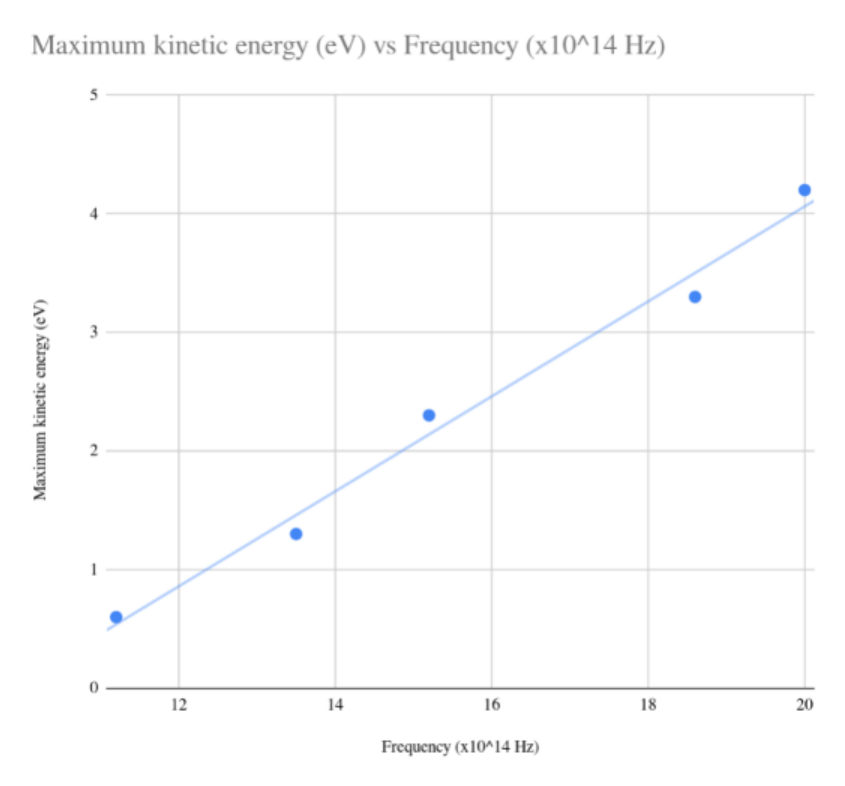
\includegraphics[width=10cm]{question_23_graph.png}
				\end{figure}

				\begin{align*}
					\text{gradient} &= \frac{4.2 - 0.6}{20.0 0 11.2} \\
							&\approx 4.09 \times 10^{-15} \, \text{eV Hz}^{-1}
				\end{align*}

				\begin{align*}
					\text{From graph;} \; f_0 &\approx 9.5 \times 10^{14} \, \text{Hz} \\
					\phi &= h f_0 \\
					     &= (4.09 \times 10^{-15})(9.5 \times 10^{14}) \\
					     &= 3.89 \, \text{eV}
				\end{align*}

			\item \textbf{Describe the difference between the spectra of the light produced by a gas discharge tube and by an incandescent lamp.}
				\subitem A gas discharge tube will only release some wavelengths of light as the electrons in the gas present jump between orbital states. An incandescent lamp produces a continuous spectrum of all wavelengths of light.


			\item \textbf{The graph shows the curves predicted by two different models, X and Y, for the electromagnetic radiation emitted by an object at a temperature of 5000 K. Identify an assumption of EACH model which determines the shape of its curve.}
				\subitem Model X is a classical wave model that states that the intensity of black body radiation is proportional to its frequency. Under this assumption, the graph approaches UV catastrophe. Model Y assumes that light consists of photons that are quantised and that energy is absorbed and emitted in packets.

			\item \textbf{The diagram shows the radiation curve for a black body radiator at a temperature of 5000 K. On the same diagram, sketch a curve for a black body radiator at a temperature of 4000 K and explain the differences between the curves.}
				\subitem The 4000 K black body radiator has a peak wavelength that is higher than the 5000 K because peak wavelength is inversely proportional to temperature. The overall intensity of the 4000K radiator is however lower.

			\item \textbf{A student performs an experiment to measure Planck’s constant, h, using a device that emits specific frequencies of light when specific voltages are applied. Data from the experiment is shown.}

				\begin{figure}[H]
					\centering
					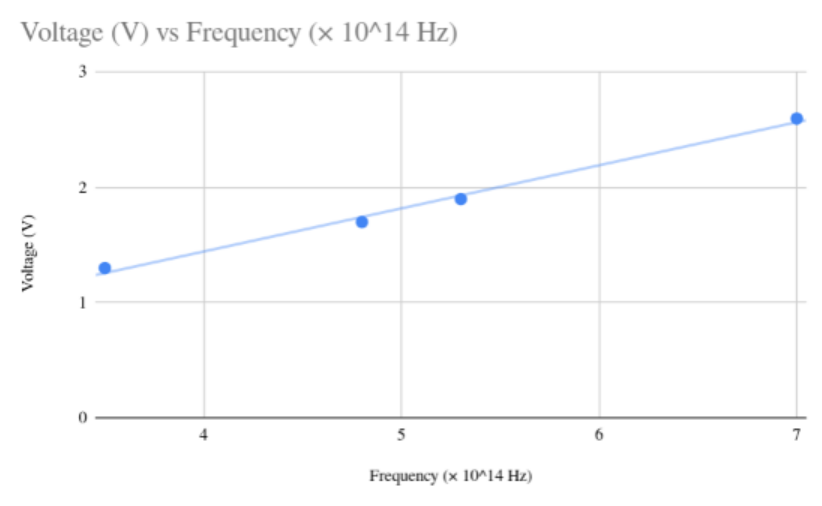
\includegraphics[width=10cm]{question_26_hsc.png}
				\end{figure}

			\item \textbf{The student proposes using data point 1 to calculate a value for Planck’s constant. Justify a better method to calculate Planck’s constant from the experimental data provided.}
				\subitem The student should instead use the gradient of voltage over frequency in their calculations. The line of best fit accounts for outliers and is a more accurate representation of the data.

			\item \textbf{Light of frequency 7.5 × 1014 Hz is incident on a calcium metal sheet which has a work function of 2.9 eV. Photoelectrons are emitted. The metal is in a uniform electric field of 5.2 NC −1, perpendicular to the surface of the metal, as shown.}
				\begin{enumerate}
					\item \textit{Show that the maximum kinetic energy of an emitted photoelectron is $3.2 \times 10−20$ J.}
						\begin{align*}
							K_\text{max} &= hf - \phi \\
								     &= 6.626 \times 10^{-34} \times 7.5 \times 10^{-14} - 2.9 \times 1.602 \times 10^{-19} \\
								     &\approx 3.2 \times 10^{-20} \, \text{J}
						\end{align*}

					\item \textit{Calculate the maximum distance, d, an emitted photoelectron can travel from the surface of the metal.}
						\subitem An emitted photoelectron will stop when work done by field = kinetic energy.
						
						\begin{align*}
							W &= qV = qEd \\
							3.2 \times 10^{-20} &= 1.602 \times 10^{-19} \times 5.2 \times d \\
							d &= \frac{3.2 \times 10^{-20}}{8.33 \times 10^{-19}} \\
							  &\approx 3.8 \, \text{cm}
						\end{align*}
				\end{enumerate}

			\item \textbf{Two experiments are performed with identical light sources having a wavelength of 400 nm. In experiment A, the light is incident on a pair of narrow slits 5.0 × 10−5 m apart, producing a pattern on a screen located 3.0 m behind the slits. How do the results from Experiment A and Experiment B support TWO different models of light? In your answer, include a quantitative analysis of each experiment.}
				\subitem Experiment A depicts Huygen's wave model of light as a self-propagating wave with a wavefront that acts as a secondary source of light. As light passes through the two slits, it is diffracted causing interference that produces the pattern seen. The distance between maxima is as follows:

				\begin{align*}
					d \sin{\ta} &= m \lambda \\
					5 \times 10^{-5} \sin{\ta} &= 1 \times 400 \times 10^{-9} \\
					\ta &\approx 0.46 \degree
				\end{align*}

				Experiment B supports the photoelectric model of light as quantised photons that act as packets of energy at a given wavelength.

				\begin{align*}
					K_\text{max} &= hf - \phi \\
						     &= 4.97 \times 10^{-19} - 4.6 \times 10^{-19} \\
						     &= 3.7 \times 10^{-20} \, \text{J}
				\end{align*}

		\end{enumerate}
\end{document}

